%************************************************
\chapter{Introduction}\label{ch:introduction}
%************************************************
\begin{refsection}[referencesCh1]
%\section{Rationale}
%
%\section{Problem statement: Overview of the nutrient pullution challenge}
%
%\subsection{Phosphorus pollution}
%
%\subsubsection{Sources}
%
%\paragraph{Livestock industry}
%\paragraph{Fertilizers application}
%\paragraph{Municipal wastewater}
%\paragraph{Industrial wastewater}
%
%\subsubsection{Environmental impacts}
%
%\paragraph{Freshewater}
%\paragraph{Marine water}
%\paragraph{Greenhouse gases emissions}
%
%\subsubsection{Approaches for the abatement of phosphorus pollution}
%
%
%\subsection{Nitrogen pollution}
%
%\subsubsection{Sources}
%\paragraph{Livestock industry}
%\paragraph{Fertilizers application}
%\paragraph{Municipal wastewater}
%\paragraph{Industrial wastewater}
%
%\subsubsection{Environmental impacts}
%
%\paragraph{Freshewater}
%\paragraph{Marine water}
%\paragraph{Greenhouse gases emissions}
%
%\subsubsection{Approaches for the abatement of nitrogen pollution}
%
%\section{Aims and scope}



%\section{Modeling approaches}
%\subsection{Process modeling}
%\subsection{Environmental geographical analysis}
%\subsection{Multi-criteria decision analysis}

\section{Rationale: Overview of the nutrient pullution challenge}
Human population is experiencing a continuous growth since end of the Black Death in the XIV century \citep{biraben1980essay}, which is at 7.8 billion as of 2020, and it is estimated to be at 9.7 billion and 10.9 billion by 2050 and 2100 respectively \citep{UNPopulationProspects}. Population growth demands increasing amounts of food, which in turn requires an efficient food production system to support this growth. In this context, the development of different technical advancements has been a key factor to increase the productivity of the food production system. Notably, crucial developments were achieved in the late modern period\footnote{The terminology used in this dissertation for the periodization of human history follows the English-language historiographical approach. It should be noted that the late modern period is referred to as the contemporary period in the European historiographical approaches.}, including the commercial production of phosphate in 1847 \citep{Samreen2019}, the development of the Haber-Bosch process for the production of synthetic nitrogen-based fertilizers in 1913 \citep{smil1999detonator}, and the mechanization of agriculture and the development of the modern intensive farming in the XX century \citep{constable2003century,nierenberg2005happier}.

Despite these advancements have increased the productivity of agriculture and farming industries, multiple environmental impacts associated with them emerges, including water scarcity, greenhouse gases emissions, nutrient pollution of waterbodies, and soil degradation, among others. These threats must be carefully addressed in order to avoid the depletion of natural resources and reach a sustainable food production system.

Focusing on the impacts derived from agriculture and farming on the nutrient cycles, it can be observed that the natural cycles of phosphorus and nitrogen have been altered these activities \citep{Bouwman2009}. Large amounts of nutrients are released into the environment in the form of synthetic fertilizers and livestock manure. Nitrogen and phosphorus are accumulated in soils, creating a nutrient legacy that is further transported to waterbodies by runoff. This process results in the eutrophication of waters, which can lead algal bloom episodes. Algal blooms are events resulting from the rapid increase of algae in a water system which can be promoted by an excess of nutrients in water, altering the normal functioning of the aquatic ecosystem. Some algal blooms can releases toxins, and they cause hypoxia as a consequence of the aerobic degradation of algal biomass by bacteria. The flow of nutrients released into the environment by anthropogenic activities is shown in Figure \ref{fig:Ch1NutrientsFlow}. 

\begin{figure}[h]
	\centering
	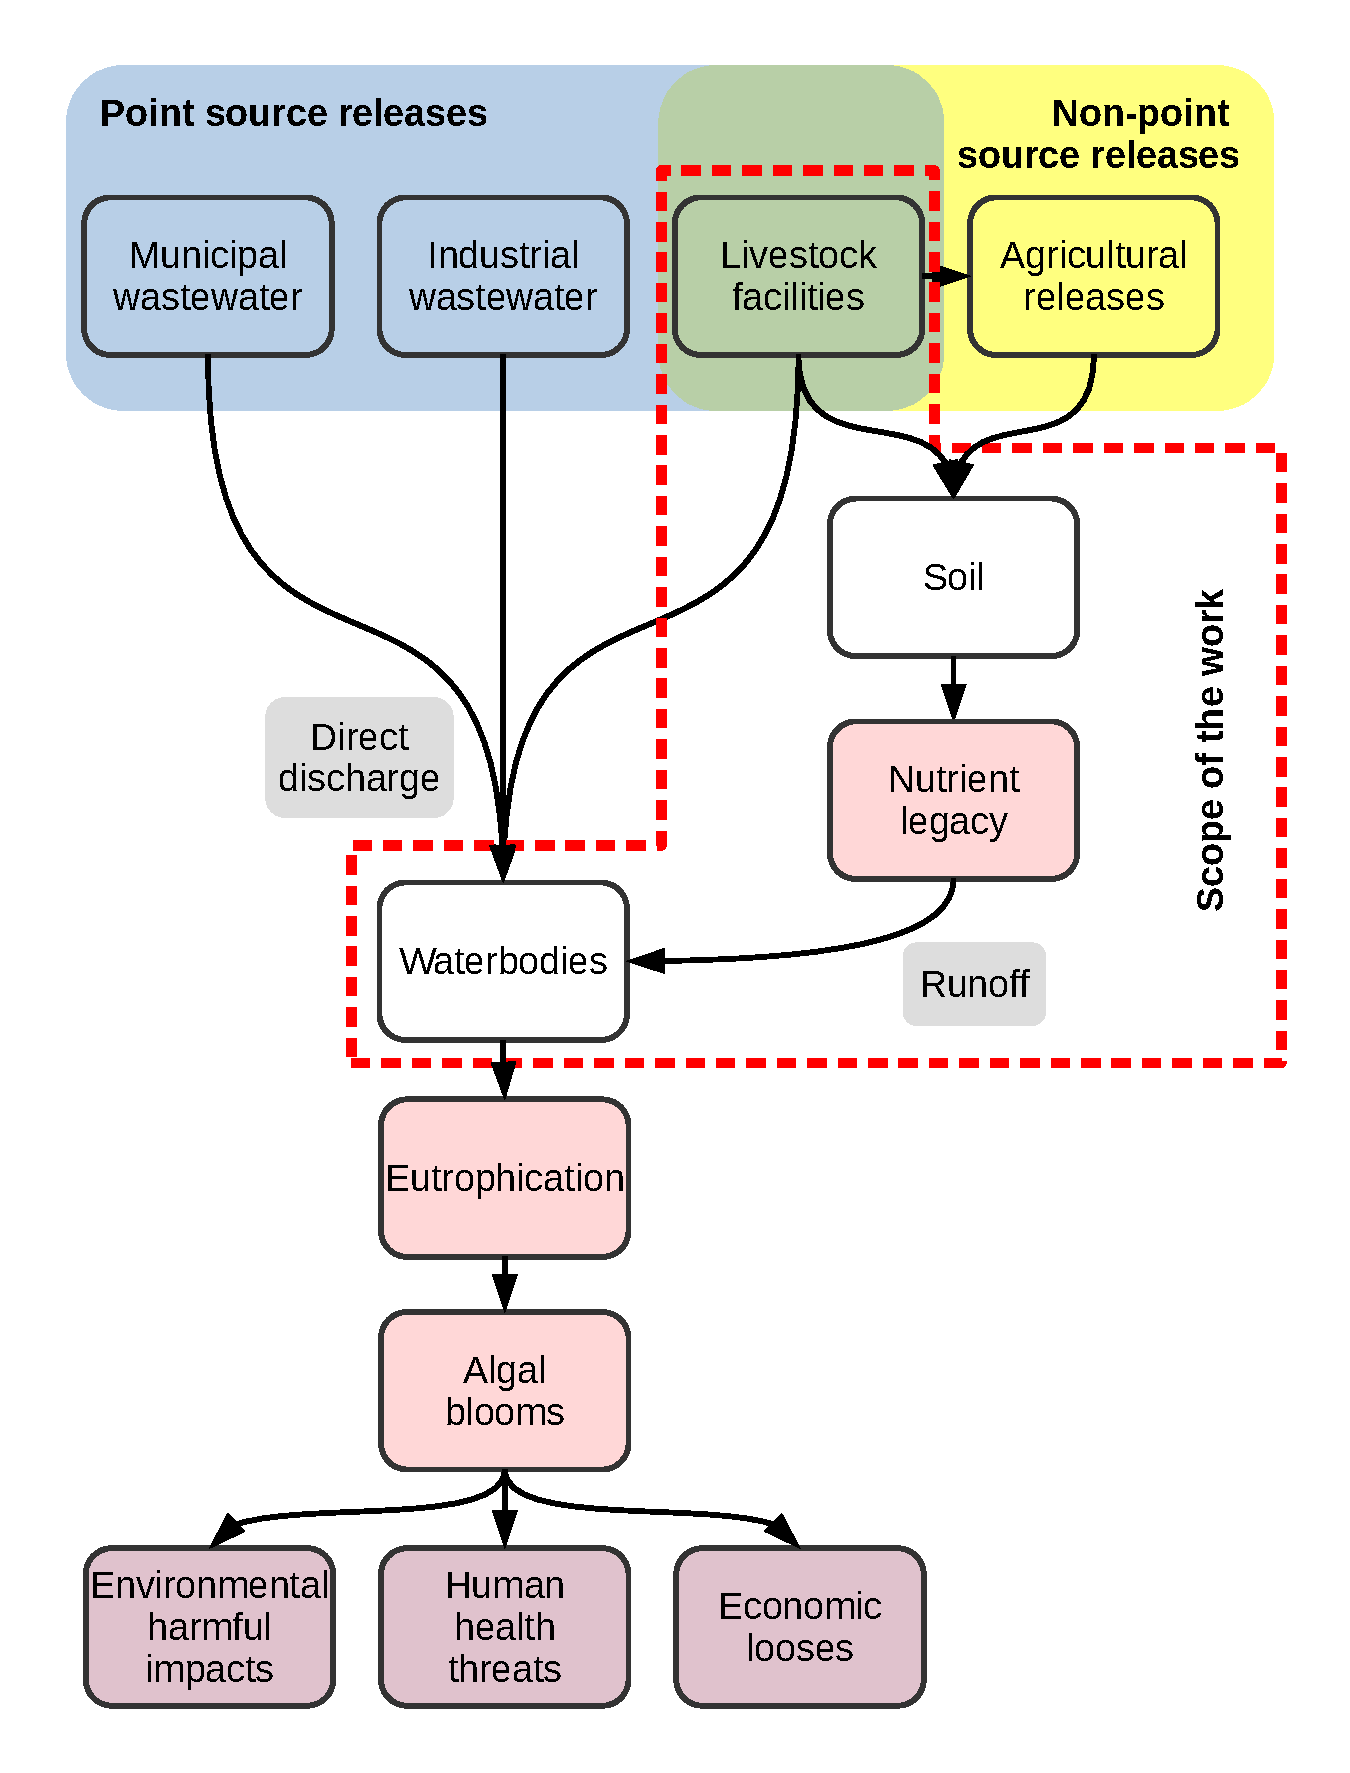
\includegraphics[width=0.85\linewidth, trim={1cm 1cm 1cm 1cm},clip]{gfx/Chapter1/IntroFig1.pdf} 
	\caption{Flow of nutrients released by anthropogenic activities.}
	\label{fig:Ch1NutrientsFlow}
\end{figure}

In addition to the environmental problems, the use of nutrients for food production also raises geopolitical concerns since phosphorus is one to the most sensitive elements to depletion. Phosphorus is a non-renewable material whose reserves are expeted to be depleted in the next 50 to 100 years, and no substitute material is currently known \citep{cordell2009story}. Conversely, synthetic nitrogen can be produced using the atmospheric N\textsubscript{2} as raw material through the Haber-Bosh process. However, nowadays this process relies on non-renewable energy sources, and therefore the production of synthetic nitrogen--based fertilizers is dependent on non-renewable resources as well.

Considering the two challenges described, i.e., nutrient pollution of waterbodies as a consequence of agricultural and farming activities, and the current dependency on non-renewable resources for the production of synthetic fertilizers, nutrient recovery and recycling is not only a desirable but also a necessary approach to develop a sustainable agricultural techniques and ensure the global food security.

Attending to the nutrient releases from livestock intensive farming facilities, known as concentrated animal feeding operations (CAFOs)\footnote{CAFO is a regulatory term defined by the US Environmental Protection Agency for large facilities where animals are kept and raised in confined situations \citep{animal_unit_definition}. This term will be used throughout the dissertation to denote the intensive livestock farming facilities studied.}, several manure management techniques are currently used. The land application of manure is a common technique that allows the recycling of nutrients as fertilizers for crops \citep{Kellog2010}. However, the increase of intensive livestock farming generates vast amounts of waste generated by CAFOs, e.g., each adult cow generates between 28 and 39 kg of manure per day, and each adult pig generates around 11.5 kg of manure per day \citep{USDAHandbook}. Commonly, manure management is based on the separation of liquid and solid phases. The liquid phase can be treated in anaerobic and/or aerobic lagoons for organic matter and pathogens removal, as well as odor control \citep{tilley2014compendium}. The obtained effluent can be used for irrigation and nutrient supplementation of crops.  The solid phase can be composted for the degradation of organic matter and pathogens removal, resulting in a solid material called compost with a larger amount of nitrogen and phosphorus available for plants, which is result of the mineralization of nutrients previously contained in organic compounds. Since compost is also a good source of organic matter for crops, it is a valuable material suitable for sale \citep{tilley2014compendium}. However, both materials, the liquid effluent obtained from the lagoons, and compost, are too bulky to be economically transported to nutrient deficient locations \citep{burns2002phosphorus}. As a result, livestock waste is usually spread in the surroundings of livestock facilities, at a detrimental cost of environment. This result in the gradual build-up of nutrients in croplands, which might lead the harmful environmental impacts previously described.

Therefore, the implementation of processes for the recovery of phosphorus and nitrogen at CAFOs is a promising alternative for abating nutrient releases and reducing the environmental footprint of livestock industry, at the time that valuable nutrient-rich materials are obtained for the redistribution of phosphorus and nitrogen to nutrient-deficient areas. There exist a number of processes for nutrient recovery from livestock waste, which can be differentiated into those technologies oriented to phosphorus recovery, including struvite precipitation, calcium-based precipitates production, coagulation-flocculation, electrochemical processes, and systems based ob phases separation; and processes focused on nitrogen recovery, such as stripping, membrane separation, waste drying coupled with ammonia scrubbing, and phases separation processes. We note that anaerobic digestion is an additional process that can be integrated for manure treatment if the generation of biomethane is pursued, and for increasing the amount of recoverable nutrients through the partial mineralization of nutrients contained in organic compounds. It must be noted that only phosphorus and nitrogen in inorganic compounds can be taken by plants, and therefore the recovery of inorganic nutrients will be the target of the processes studied in this thesis.

The multiple processes for the recovery of phosphorus and nitrogen from livestock waste differ in aspects such as recovery efficiency, processing capacity, capital and operating costs, and final products obtained. Therefore, a detailed analysis of each CAFO must be performed in order to select the optimal nutrient recovery system attending to type factors such as the type and amount of waste to be processed, the environmental vulnerability to eutrophication od each region, the current or potential installation of anaerobic digestion systems, etc. Additionally, in the decision-making process these factors have to be prioritized to select the most suitable process for each particular facility, i.e., in regions with a low risk of eutrophication, more economical processes for nutrient recovery could be installed in even though their recovery efficiency may be lower than other alternatives. Conversely, regions at severe eutrophication risk require highly efficient nutrient recovery systems that may incur in larger investment and operating expenses. In order to perform a systematic evaluation of CAFOs and their context, we introduce a multi-criteria decision analysis (MCDA) framework integrating geospatial environmental data regarding eutrophication risk at the subbasin level and data from the techno-economic analysis of the processes studied. 

Attending to the regulatory aspect, nowadays most of the efforts for abating of nutrient releases into the environment and mitigating the eutrophication of waterbodies are focused in the limitation of fertilizer application in croplands. The application of fertilizer and manure for nitrogen supplementation in the European Union (EU) is currently regulated by the Nitrates Directive (91/676/EEC) \citep{GRIZZETTI2021102281}. Regarding the limitations for phosphorus application, these are defined at national level. Several European countries have implemented application standards based on the different crops and materials used as fertilizers. Generally, phosphorus application limits are more restrictive in northwestern Europe \citep{amery2014agricultural}. It can be observed that nutrient application is limited either in the form of synthetic fertilizers or manure application. However, at present there is a lack of regulation regarding livestock waste treatment \citep{Piot_Lepetit2012}. New efforts for the adoption of bio-fertilizers obtained from organic waste are being currently performed in the development of the "Integrated Nutrient Management Plan" (INMAP), which is part of the part of the EU Farm-to-Fork strategy and part of the Circular Economy Action Plan. INMAP should propose actions to promote the recovery and recycling of nutrients, as well as the development of markets for recovered nutrients \citep{ESSP2021, CircularEconomyActionPlan}. In this regard, a new regulation for fertilizer products has been released in 2019 (EU 2019/1009), moving struvite and other biofertilizers from the category of waste to fertilizers, establishing a regulatory framework for their use and trade.

In the United States, CAFOs are regulated under the Clean Water Act as point source waste discharge. This regulation sets the need of permits for discharging pollutants to water, called National Pollutant Discharge Elimination System (NPDES) permits, including the release of nitrogen of phosphorus. This permit must include the necessary provisions for avoiding the harmful effects of the discharges on water and human health \citep{NPDE_basics}. The development and implementation of a Nutrient Management Plan (NMP) is a required element to get a NPDES permit. This document must identify the management practices to be implemented at the CAFO to protect natural resources from nutrient pollution. Land spreading of manure can also be regulated by the NPDES permits, establishing soil nutrient concentration limits and the yearly schedule for manure application. However, no specific methods or processes are defined under federal regulation \citep{NPDESforCAFO}. Regarding the use of the recovered nutrients, products obtained from nutrient recovery processes could be classified as waste ny the Clean Water Act, preventing the application of these materials on croplands \citep{NACWA503}. However, U.S. Environmental Protection Agency (US EPA) determined that, although these products could not be directly applied to land under the current regulation, they can be sold as a commodity to be outside of the Clean Water Act restrictions coverage. Moreover, US EPA acknowledges that highly refined and primarily inorganic products (such as struvite) could be outside of the scope of these restrictions \citep{CNP503}. However, further regulation is needed for defining the products obtained from nutrient recovery processes and to clearly state the conditions for their use as fertilizers on croplands.

Considering the previously described aspects, we note that the regulation of the products obtained from nutrient recovery systems is not totally developed yet, although important efforts are being performed in order to set a comprehensive regulatory framework for the recycling of phosphorus and nitrogen. Furthermore, no regulation regarding the implementation of nutrient recovery processes has been developed either in the EU and the US. However, both regions have developed programs to study and promote the implementation of other technologies for the treatment of livestock waste, specially the deployment of anaerobic digestion systems. These programs could be a guideline for the development of nutrient recovery plans at CAFOs. In this regard, we have studied the impact of the implementation of nutrient recovery systems in the economy of CAFOs, either considering the deployment of standalone nutrient recovery processes or integrated with anaerobic digestion for the production of electricity. Moreover, incentive policies have been analyzed to minimize the negative impact of nutrient recovery on CAFOs economy using the Great LAkes area as case study. In addition, the fair distribution of monetary resources when limited budget is available has been studied using the Nash allocation scheme. 

An overview of the main topics studied in this thesis can be observed in Figure \ref{fig:Ch1WorkThesis}. This work pretends to analyze strategies for promoting effective nutrient recycling addressing studies on the technical, environmental and economic dimensions involved, pursuing the development of sustainable food production paradigm.

\begin{figure}[h]
	\centering
	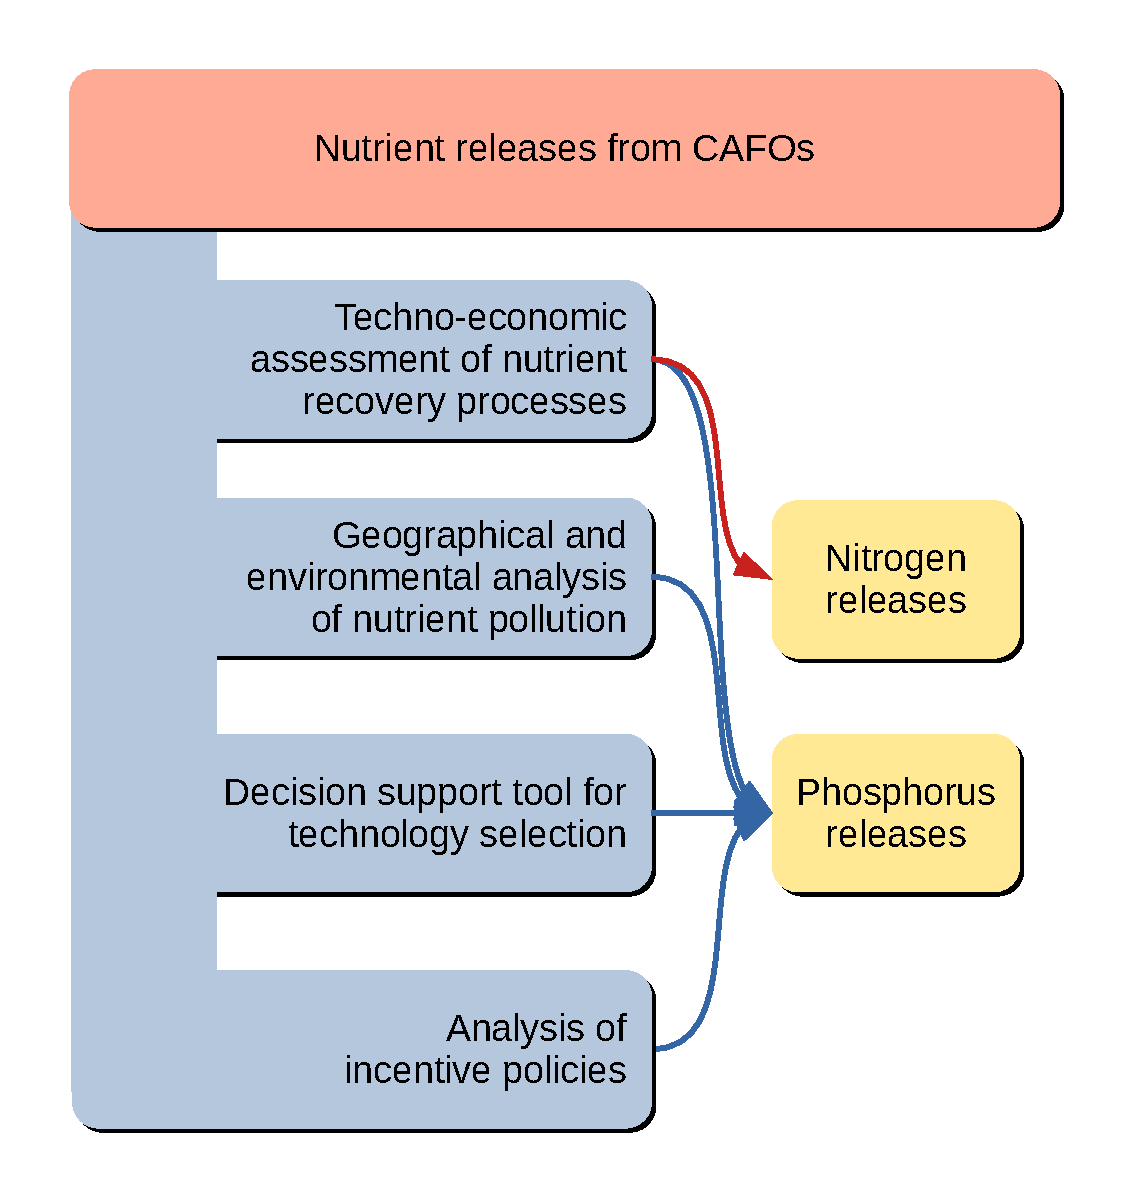
\includegraphics[width=0.7\linewidth, trim={1cm 1cm 1cm 1cm},clip]{gfx/Chapter1/IntroFig2.pdf} 
	\caption{Main topics covered in this work.}
	\label{fig:Ch1WorkThesis}
\end{figure}. 


%\section{Scope and objectives of the thesis}
%This thesis seeks to promote the recovery and recycling of nutrients contained in livestock waste by identifying the most appropriate technologies for phosphorus and nitrogen recovery at cattle and swine CAFOs, assessing the potential nutrient releases abatement that could be achieved by the deployment of these systems and analyzing incentive policies for their effective implementation at livestock facilities. Moreover, we introduce a systematic framework for evaluating and selecting the most suitable nutrient recovery system at CAFOs considering geospatial environmental vulnerability to nutrient pollution. 
%\paragraph{Objective I:} To perform a review of the state-of-the-art of the processes for phosphorus and nitrogen recovery from livestock waste, identifying those processes whose implementation at CAFOs is feasible from a techno-economic perspective.
%\paragraph{Objective II:} To identify environmental indicators for nutrient pollution, and use  them to  assess the potential for the abatement of phosphorus releases by deploying the processes previously selected at livestock facilities at subbasin spatial resolution.
%\paragraph{Objective III:} To develop a decision-support system for the evaluation and selection of nutrient recovery systems at livestock facilities integrating techno-economic data of the nutrient recovery technologies and environmental vulnerability to nutrient pollution information determined through a tailored geographic information system (GIS) in order to select  the most suitable system for each particular livestock facility.
%\paragraph{Objective IV:} To design and analyze potential incentive policies for the deployment of phosphorus recovery technologies at livestock facilities, as well as to study the fair allocation of limited monetary resources.

\section{Approaches for processes modeling}
Process modeling, defined as the mathematical modeling and simulation of systems, falls under the scope of Process System Engineering (PSE) discipline. These systems include physical, chemical, and/or biological operations. Process modeling forms the foundation for other activities involved in the scope of PSE, including process design, optimal scheduling and planning of the systems operations, and process control \citep{STEPHANOPOULOS20114272}.

Different modeling techniques have been developed to mathematically describe and represent systems from different domains, including but not limited to the chemical, biochemical, agrochemical, food, and pharmaceutical domains of engineering \citep{PISTIKOPOULOS2021107252}. An overview of the main modeling techniques is shown in the next sections based on the classification proposed by \citet{MARTIN201216}.

\subsection{Short-cut methods}
These type models are the most basic approach to process modeling. They are based on mass, energy, and momentum balances, and can be embedded in other models, such as supply chain models.

\subsection{Rules of thumb}
This approach is based on industrial operational data. It provides typical ranges for operating and design values, reflecting the actual parameters of the systems modeled. However, the use of these models is constrained by the availability of data. Compendiums of rules of thumb for different systems can be found in \citet{couper2005chemical, hall2012rules, sadhukhan2014biorefineries}.

\subsection{Dimensionless analysis}
This methodology is based on dimensionless groups that describe the performance of a particular system. These models are able to capture the physical meaning of the modeled processes, and they are specially useful to capture scale-up and scale-down issues \citep{szirtes2007applied}.

\subsection{Mechanistic models}
This approach relies on first principles for systems modeling, as short-cut models. However, mechanistic models rely in more detailed first principles such as the underlying chemistry, physics or biology that governs the behavior of a particular system. Chemical \citep{loeppert1995chemical} and phase \citep{brignole2013phase} equilibrium models, kinetic models \citep{buzzi2009kinetic}, population balances \citep{ramkrishna2000population}, and computer fluid dynamics (CFD) \citep{anderson1995computational} fall under this category.

\subsection{Surrogate models}
These models aim at developed simplified models from data obtained from rigorous mechanistic models. This approach is widely used for embedding system models into other applications such as process control or supply chain design. Surrogate models building has been systematized into four steps, i.e., design of experiments (DOE), running the rigorous models at the sampling points designated by the DOE, construction of the surrogate model, and validation of the model obtained \citep{queipo2005surrogate}.

Polynomial regression models, in which the relationship between the variables is expressed using a polynomial function, are one of the most basic types of surrogate models. In the case of polynomial regression models involving multiple variables, the optimal variables to be addressed within the pool of variables considered can be determined by using machine learning-based tools such as ALAMO \citep{wilson2017alamo}, ensuring an optimal trade-off between model accuracy and complexity. Other types of surrogate models are Kriging models, which estimate the relationship between variables as a sum of a linear model and a a stochastic Gaussian function representing the fluctuations of data \citep{quirante2015rigorous}, and artificial neural networks (ANN), which are based on  generating an input signal as the summation of all the
weighted inputs, which is through nodes containing a transfer function. Nodes are connected by edges with assigned weights that adjust the signals transmitted between nodes. Nodes are structured in layers, in a way that nodes receive signals from nodes of the preceding layer, and if the output of the node is above a threshold value defined by the transfer function, sends the output signal to the next layer \citep{himmelblau2000applications}.

\subsection{Experimental correlations}
As the surrogate models, experimental correlations are models built using data of the systems represented, but converserly to those one, experimental correlations are built using data  from experimental results. Similarly to the rules of thumb, the accuracy of these models is limited by the availability of data, and they are only applicable to the range of operating conditions of the data used for constructing the model.

\section{Approaches for decision-support systems}
Decision-making activities require to analyze multiple relevant criteria for each course of action. Since criteria often conflict each other, each decision-making process requires the balancing of criteria, prioritizing some criteria over other through the use of some criteria weighting scheme. This procedure requires managing a vast amount of information of conflicting nature, leading to a complex decision-making process. Therefore, different approaches generally called multiple-criteria decision analysis (MCDA) have been developed to explicitly structure and solve decision problems. MDCA aim is to integrate criteria assessment with value judgment to analyze and compare the different available alternatives, identifying the best solution for the decision-making context studied. However, it must be highlighted that a certain grade of subjectivity might exist is several steps of MCDA, such as the choice of the set of criteria that are considered relevant for a particular problem. Therefore, the solution proposed by any MCDA approach must be analyzed considering the assumptions made for building the problem. As a result, MCDA seeks to structure problems with multiple conflicting criteria, and providing justifiable and explainable solutions to guide decision-makers facing such problems. The solution of a multiple-criteria decision-making problem can defined as a unique solution representing the most suitable alternative from the set of potential alternatives for a particular decision-making context, or a subset of satisfactory alternatives \citep{belton2002multiple}.

A MCDA problem can be articulated in different stages, starting with the problem definition and structuring. At this stage, the goals, constraints, and stakeholders comprising the problem are defined, as well as the different solution alternatives. Based on this information, a model can be built for the assessment and comparison of alternatives. This stage includes the definition of the relevant criteria used for alternatives comparison, their relative priority, and the criteria evaluation system. Finally, the information retrieved by the model can be used for making informed decisions. {\color{red}{figure?}}

Multi-criteria decision-making problems can be divided into Multi-Attribute Decision Analysis (MADA), which are discrete choice problems where the number of alternatives is finite, and Multi-Objective Decision Analysis (MODA), that are mathematical programming problems that consider infinite number of alternatives. However, we note mathematical programming techniques are not limited to formulating and solving problems with infinite alternatives, but they can also be used for dealing with discrete decision-making problems \citep{giove2009decision}. {\color{red}{figure?}}

\subsection{Multi-Attribute Decision Analysis (MADA)}

In the case of problems consisting of a finite number of alternatives, the suitability of each alternative to the problem given can be measured through its performance according to the multiple criteria considered. A large number of MCDA approaches have been (and are currently being) developed for discrete choice problems, including methods based on value functions (Multi-Attribute Value Theory methods, MAVT) and outranking methods.

\subsubsection{Multi-Attribute Value Theory (MAVT)}
\paragraph{Indicator-based methods}
In this approach, an indicator-based methodology is used for alternatives comparison. The relevant criteria considered in the decision-making process are a normalized to a common scale to allow criteria comparison using a utility or value function. A number of utility functions have been proposed in the literature, including standardization, min-max, and target utility functions \citep{HandbookCompositeIndicators}. 
The normalized criteria 
%are weighted to set the relative importance of each criterion, prioritizing some criteria over others. In the last step, weighted criteria 
are weighted and aggregated to build a composite index, prioritizing some criteria over others. Different aggregation schemes denote different degrees of compensability between indicators, i.e. a deficit in one criteria can be fully, partially, or not compensated by a surplus in other criteria \citep{MarcoCinelli2020}. Additive weighting aggregation is a full compensatory method, while geometric and  harmonic aggregation methods are partial  compensation schemes. Other aggregation schemes include geometric averaging, which is a non-compensatory method, and the Choquet integral \citep{marichal2000determination}. The composite index obtained is a single numerical value that can be used to score and rank the proposed alternatives based on their suitability to the criteria considered. 

%Uncertainty can be addressed with MAVT methods using different techniques, such as sensitivity analysis, bayesian approaches, and fuzzy set theory methods. 
A major source of uncertainty in indicator-based methods is the value of criteria weights. This can be addressed using the stochastic multi-criteria acceptability analysis (SMAA) method. SMAA is a sensitivity analysis method that address the uncertainty of criteria weights value exploring the feasible space of weights through the Monte Carlo method. Details about the SMAA approach can be found in \citet{tervonen_implementing_2007}.

%In this thesis, and indicator-based methodology has been used to assess and select phosphorus recovery technologies based on technical, environmental, and economic criteria combined in a composite index.

%Another MAVT approaches include Analytic Hierarchy Process (AHP) and the Ideal Point Methods. 
\paragraph{Analytic Hierarchy Process (AHP)}
Analytic Hierarchy Process (AHP) decomposes the decision problem in multiple simpler sub-problems. These sub-problems are hierarchized are independently analyzed. These sub-problems are solved through the pairwise comparison of the alternatives, obtaing numerical indexes that can be used to compare their performance. Finally a numerical weight (priority) is assigned to each element of the hierarchy, and they are used for aggregating the indexes obtained by each alternative in a final numerical value that can be used to score the overall performance of each alternative accordingly to the set of criteria considered \citep{saaty2000fundamentals}. 

\paragraph{Ideal Point methods}
Ideal Point methods set an optimal solution, that represent a utopia point where all criteria values are optimal. The performance of each alternative is evaluated through a composite index, that can be constructed using the techniques previously described. The alternatives are ranked based on their relative distance relative to the optimal solution. One of the most Ideal Point methods is TOPSIS \citep{hwang1995multi}.



%common scale to allow each criteria to be compared with the others.
%such as ELECTRE or PROMETHEE, analytic hierarchy process (AHP), fuzzy models, and indicator-based approaches, among others. In this thesis, and indicator-based methodology has been used to assess and select phosphorus recovery technologies based on technical, environmental, and economic criteria combined in a composite index. The construction of this composite index is composed of three steps: criteria normalization, weighting, and aggregation. Since each criteria has a different range of potential values, they must be normalized to a common scale to allow each criteria to be compared with the others. To account for robustness and resiliency of the solutions obtained, different normalization techniques have been studied. The normalized criteria are weighted to set the relative importance of each criterion, prioritizing some criteria over others. In order to avoid the risk of biasing the decision-making procedure setting arbitrary
%values for the weighting, a stochastic multi-criteria acceptability analysis (SMAA) is used to explore the weights space through the Monte Carlo method. Details about the SMAA approach can be found in \citet{tervonen_implementing_2007}. Finally, weighted criteria are aggregated to build the composite index. Different aggregation schemes denote different degrees of compensability between indicators, i.e. a deficit in one criteria can be fully, partially, or not compensated by a surplus in other criteria \citep{MarcoCinelli2020}.  Similarly to the normalization stage, different aggregation methods, including one full compensation and two partial compensation schemes are evaluated to achieve a robust solution.

\subsubsection{Outranking methods}
Outranking methods are based on the pairwise comparison of the alternatives for each criterion considered, determining the preferred alternative for each of the criteria. Preference information about all criteria is aggregated to establish evidence for selecting one alternative over another. These methods indicate the dominance of one alternative over another, but they do not quantify the performance gap between the alternatives compared \citep{giove2009decision}. Some of the most popular outranking methods are ELECTRE I \citep{roy1968classement}, II \citep{roy1973methode}, and III \citep{roy1978electre}, and PROMETHEE \citep{vincke1985preference}.

\subsubsection{Multi-Objective Decision Analysis(MODA)}

%Alternatively, p
Problems consisting of an infinite number of solutions require multi-objective mathematical programming (optimization) techniques to be solve. These problems are subjected to a number of equality and/or inequality constraints restricting the solutions that are feasible, and the multiple conflicting criteria are combined in an objective function. This objective function represents the improving level of the criteria, and it will be minimized or maximized for selecting the best solution that represents the optimal trade-off between the different conflicting criteria. In this thesis, this technique has been employed for selecting the operating conditions of processes for the recovery of nutrient, energy and biomethane from livestock waste, as it is shown in Chapters \ref{ch:PhosphorusTechs} and \ref{ch:BiogasUpgrading}. Other approach for solving multi-objective mathematical programming problems is to set a priory targets for different criteria, or combinations of criteria, that are considered satisfactory, obtaining the problem solution by minimizing the deviations from these goals. Mathematical programming problems can be also classified according to the use of linear or nonlinear equations, and continuous and/or discrete variables.

\paragraph{Linear programming}
Linear programming (LP) refers to those mathematical programming problems based on linear equations and continuous variables. A linear programming problem can be expressed as shown in Eq  \ref{eq:IntroEq1},  where $x$ is an n-vector, $A$ is a mxn matrix, $c$ is the n-vector of cost coefficients, and the right-hand side $b$ is an m-vector \citep{grossmann2021advanced}.

\begin{align}
	\min \quad & Z=c^{T}x \nonumber\\
	\textrm{s.t.} \quad & Ax=b \label{eq:IntroEq1}\\
	&x \geq 0  \nonumber  
\end{align}

The two most widely used methods to solve LP problems are the Simplex algorithm \citep{murty1983linear} and interior-point methods \citep{POTRA2000281}. The Simplex method is more efficient for solving problems with thousands of variables and constraints, while interior-point performs better on very large scale and sparse problems \citep{grossmann2021advanced}. The most representative commercial solvers such as CPLEX, GUROBI, or XPRESS implement both methods.

\paragraph{Nonlinear programming}
Nonlinear programming (NLP) refers to those mathematical programming problems containing nonlinear equations, either in the constrains or in the objective function, and continuous variables. A nonlinear programming problem can be expressed as shown in Eq  \ref{eq:IntroEq2}, where $x$ is a n-vector, $f(x)$ is the objective function of the problem, $h(x)$ is the set of equality constraints and $g(x)$ is the set of inequality constraints. \citep{floudas1995nonlinear}.

\begin{align}
\label{eq:IntroEq2}
\min \quad & f(x) \nonumber\\
\textrm{s.t.} \quad & h(x)=0\\
& g(x) \leq 0 \nonumber\\
&x \in X  \subseteq \Re^{n} \nonumber
\end{align}

\section{Approaches for geospatial environmental assessment}
Human actions, from food production\citep{foster2007environmental} to cloud computing \citep{di2017can}, result in harmful impacts endangering and deteriorating the environment. The development of mitigation measures to reduce the environmental footprint of anthropogenic activities requires the previous understanding and quantification of the environmental impacts associated to each sector. This process, called environmental impact assessment (EIA), involves the analysis of multi-disciplinary information, including environmental, physical, geological, ecological, economic, and social data \citep{gharehbaghi2018gis}. Since EIA aims to evaluate the environmental impact of an activity on a particular geographical location, all these data have a common geographic component, becoming geospatial data.

Geospatial data can be managed and analyzed through specific systems denoted as geographic information system (GIS). GIS is a key tool for EIA that uses the geographic component of geospatial data as an integrative framework that provides the ability to analyze and map descriptive information of the locations studied. The geographic component of data is the key element of GIS systems, since the spatial (or spatio-temporal) location is used as a key to relate other descriptive information. From the perspective of EIA, this information can be analyzed, interpreted, and mapped to determine the vulnerability level of each location to a particular environmental threat, find relationships between human activities and environmental damages, measure the performance of mitigation and remediation processes, etc. {\color{red}{figure?}}

The combination of GIS, EIA, and methods for the analysis of multi-dimensional information, such as MCDA, provides tools for the development of sustainable strategies for the transition to a sustainable paradigm for human growth. In this regard, the development of a sustainable, reliable, and resilient water, energy and food nexus is a major issue for food security and environmental protection.

\section{Thesis outline}
This dissertation is structured in three parts. Part I is devoted to the study of phosphorus management and recovery, Part II address a techno-economic assessment of the technologies for nitrogen recovery, and Part III conduct a research for determining the best combination of units for biomethane production in order to integrate biogas production and nutrient recovery processes.

\subsection{Part I - Phosphorus management and recovery}
\paragraph{Chapter \ref{ch:PhosphorusTechs} - Technologies for phosphorus recovery.} This chapter performs a review of the main processes for phosphorus recovery from livestock waste, identifying the most promising processes to be deployed at CAFOs using a mixed-integer nonlinear programming model.

\paragraph{Chapter \ref{ch:Struvite} - Assessment of phosphorus recovery through struvite precipitation.} This chapter study the mitigation of phosphorus releases through the deployment of struvite precipitation systems in the watersheds of the contiguous Unites States. Specific surrogate models to predict the production of struvite and calcium precipitates from cattle leachate were developed based on a detailed and robust thermodynamic model. In addition, the variability in the organic waste composition is captured through a probability framework based on Monte Carlo method.

\paragraph{Chapter \ref{ch:Tool} - Geospatial environmental and techno-economic framework for sustainable phosphorus management at livestock facilities.} This chapter presents a decision support framework, COW2NUTRIENT (Cattle Organic Waste to NUTRIent and ENergy Technologies), for the assessment and selection of phosphorus recovery technologies at CAFOs based on environmental information on nutrient pollution and techno-economic criteria. This framework combines eutrophication risk data at subbasin level and the techno-economic assessment of six state-of-the-art phosphorus recovery processes in a multi-criteria decision analysis (MCDA) model. We aimed to provide a useful framework for the selection of the most suitable P recovery system for each particular CAFO, and for designing and evaluating effective GIS-based incentives and regulatory policies to control and mitigate nutrient pollution of waterbodies.

\paragraph{Chapter \ref{ch:Policies} - Analysis of incentive policies for phosphorus recovery.} This chapter conduct a research on the design and analysis of incentive policies using the COW2NUTRIENT framework for the implementation of phosphorus recovery technologies at CAFOs minimizing the negative impact in the economic performance of CAFOs. Moreover, the fair allocation of monetary resources when the available budget is limited is studied using the Nash allocation scheme.

\subsection{Part II - Nitrogen management and recovery}
\paragraph{Chapter \ref{ch:NitrogenTechs} - Multi-scale techno-economic assessment of nitrogen recovery systems for swine operations.} This chapter performs a review of the main processes for nitrogen recovery at intensive swine operations. A multi-scale techno-economic analysis is performed to estimate the capital and operating costs for different treatment capacities, identifying the most promising processes.

\subsection{Part III - Nitrogen management and recovery}
\paragraph{Chapter \ref{ch:BiogasUpgrading} - Optimal technology selection for the biogas upgrading to biomethane.} This chapter performs a systematic study of different biogas upgrading to biomethane processes in order to identify the optimal process attending to the particular characteristics of the biogas produced from livestock manure. Food waste and wastewater sludge are also included for comparison. We aimed to determine the optimal biomethane production processes for the potential combination of biomethane production and nutrient recovery processes into an integrated resources recovery facility.
%The case study demonstration consists of implementing and assessing the sustainable performance of nutrient and energy recovery at 2,217 CAFOs located in the U.S. Great Lakes area (i.e., Minnesota, Indiana, Ohio, Pennsylvania, Wisconsin, and Michigan).

%technic, economic, and environmental dimensions of nutrient recovery at CAFOs have been integrated in a decission support system 
\section*{Bibliography}
\addcontentsline{toc}{section}{Bibliography}

\printbibliography[heading=none]
\end{refsection}